\begin{figure}
    \centering
    \begin{minipage}{.5\textwidth}
      \centering
      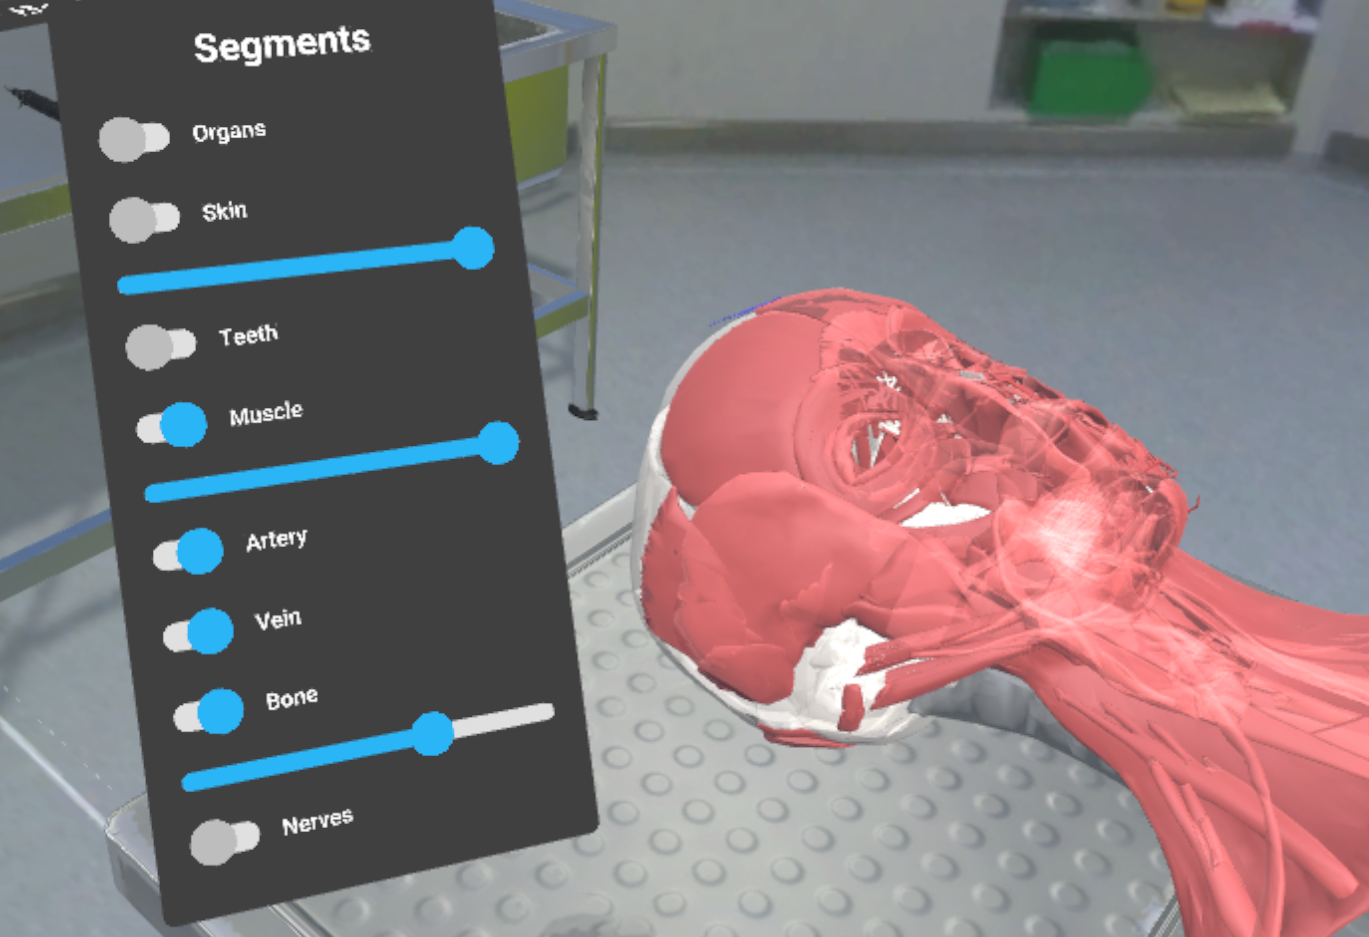
\includegraphics[width=0.95\linewidth]{images/implementation/features/visualization/segments_1.png}
      \captionof{figure}{Segment enabled}
      \label{fig:test1}
    \end{minipage}%
    \begin{minipage}{.5\textwidth}
      \centering
      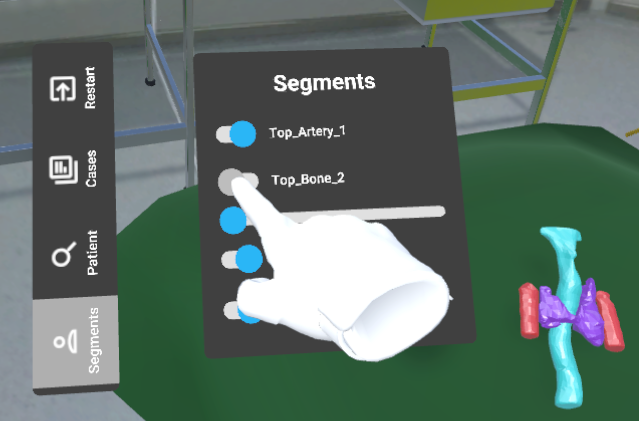
\includegraphics[width=0.95\linewidth]{images/implementation/features/visualization/segments_2.png}
      \captionof{figure}{Segment disabled}
      \label{fig:test2}
    \end{minipage}
    \end{figure}

\begin{figure}[ht!]
    \centering
    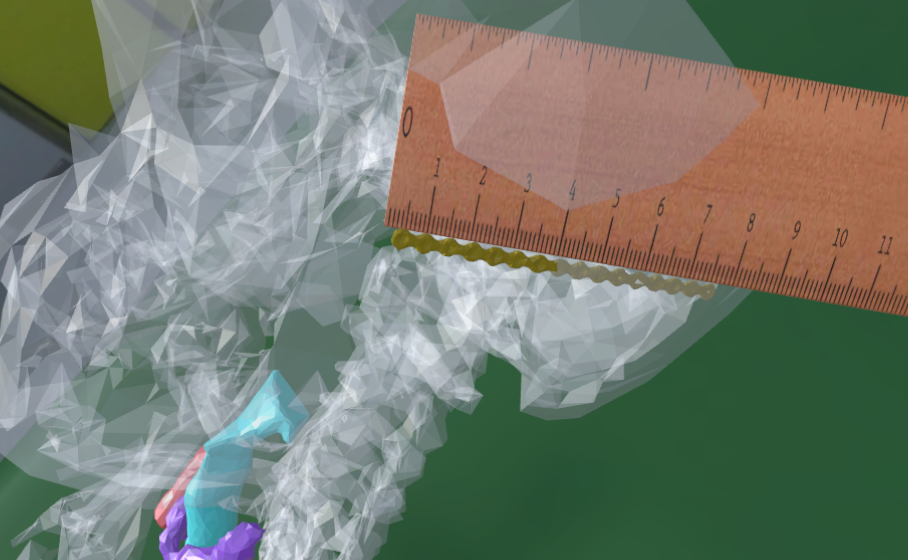
\includegraphics[width=\linewidth]{images/implementation/features/visualization/ruler.png}
    \caption{\label{fig::FeatureRuler} Ruler for Checking distances}
\end{figure}

\input{sections/4_implementation/features/visualization/explodeview.tex}